\section{Muestreo sub-Nyquist}
En este apartado se emplea la misma señal que se desarrolló en la sección anterior:

\begin{align*}
    x_5(t) = A_{max} \cdot [1+cos(2\pi \cdot f_m \cdot t)] \cdot cos(2\pi \cdot f_{port}\cdot t)
\end{align*}

\noindent donde $f_{port} = 2 \cdot f_{in}$ y $f_m = 0.2 \cdot f_{port} $. Utilizando $f_{in} = 0.8 \cdot f_p = 17.64kHz$. De este modo: $f_{port} = 35.28kHz$ y $f_m = 7kHz$.

\subsection{Introducción teórica}
Se plantea realizar el muestreo de la señal sin que ocurra aliasing. Notar que no se solicita recuperar la señal original, dado que bajo estas condiciones no es posible hacerlo. Lo que detallará a continuación se suele llamar 'muestreo de señales pasa-banda'.

Si se dispone de una señal que dispone de un ancho de banda $B$, tal que su espectro es no nulo en $f_c-B/2 < f < f_c+B/2$ (recordar que a excepción que se indique lo contrario estamos trabajando con señales reales, por lo que el módulo del espectro ha de ser par y la fase impar, de este modo lo que se indique para el semi-eje positivo en magnitud ocurre para el negativo también):

\begin{figure}[H]
  \centering
  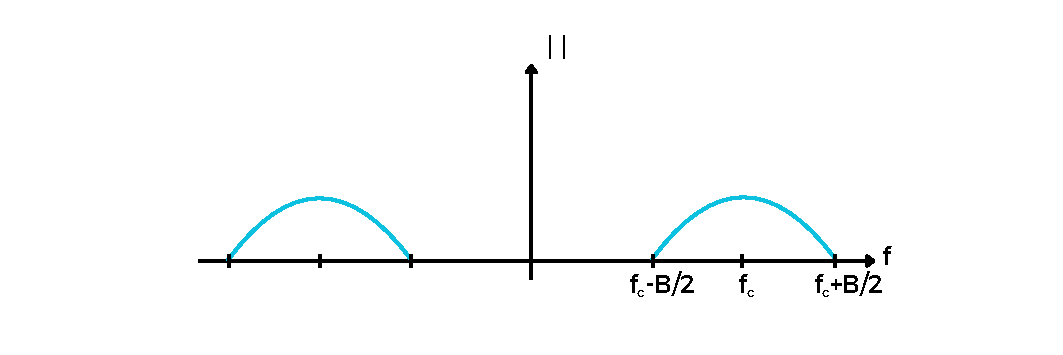
\includegraphics[width = \textwidth]{Imagenes/7_Sub_nyq/esquema_inicial.pdf}
  \caption{Esquema inicial}
  \label{fig: 7 esquema inicial}
\end{figure}


\noindent Si realizamos un muestreo (independientemente del tipo) se obtendrán una serie de réplicas del espectro original en función de la frecuencia de muestreo $f_s$. En general, las replicas se encuentran centradas en $n \cdot f_s \pm f_c$, con $n\in \mathbb{Z}$. Cuando tratamos la frecuencia de Nyquist, se dispone del caso límite para que la primera imagen se superponga con la de banda base:

\begin{figure}[H]
  \centering
  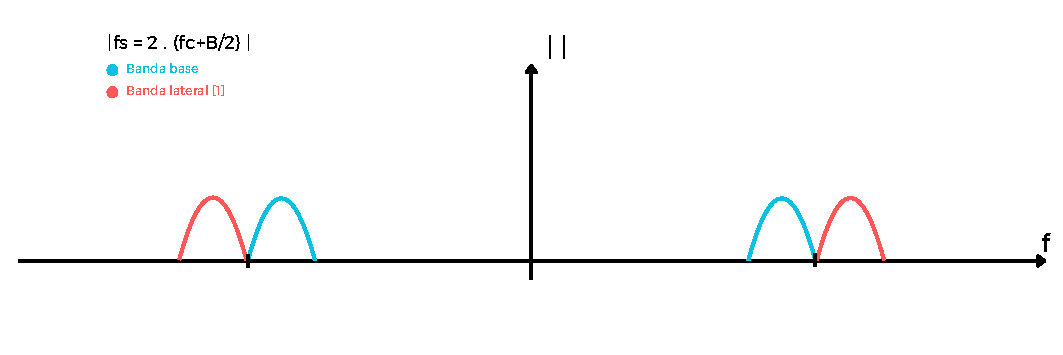
\includegraphics[width = \textwidth]{Imagenes/7_Sub_nyq/cond_nyq.pdf}
  \caption{Condición de Nyquist.}
  \label{fig: 7 condicion de nyquist}
\end{figure}


Si continuamos disminuyendo la frecuencia, se superpondran las imágenes con las componentes originales, produciendo lo que se conoce como aliasing. Sin embargo, llegada una frecuencia deja de haber aliasing, provocando que se dispongan de 2 réplicas del espectro en banda base:

\begin{figure}[H]
  \centering
  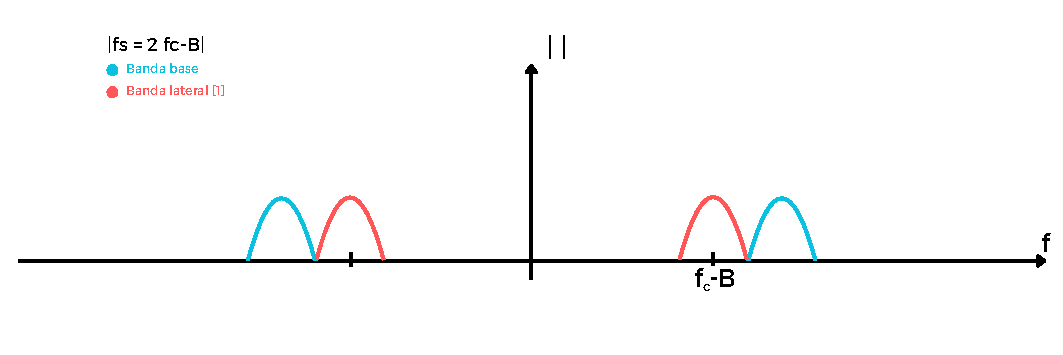
\includegraphics[width = \textwidth]{Imagenes/7_Sub_nyq/m_2.pdf}
  \caption{1 replica en espacio libre.}
  \label{fig: 7 replica en espacio libre}
\end{figure}


Si se disminuye aún más la frecuencia la frecuencia ocurrirá lo mismo, llegará un punto donde habrá nuevamente superposición, pero habrá otro intervalo donde esta dejará de ocurrir, aumentando la cantidad de imágenes en banda base. 


Por obvias razones existe un límite de la cantidad de imágenes que caben en esta banda dado por:  $m_{val} = [(f_c-B/2)/B] = [f_c / B + 1/2]$, donde $[.]$ representa al operador parte entera.

Se puede generalizar los rangos $[{{f_s}^m}_{min};{{f_s}^m}_{max}]$, donde m representa la cantidad de réplicas en la banda base. Comencemos por el límite inferior. Si se dispone de \emph{m} imágenes en la banda base, el caso a analizar ocurre cuando la imagen de la banda m+1 está por superponerse con la original. De este modo si se iguala la posición lateral izq de la imagen y la derecha de la original se obtiene el límite buscado:

\begin{align*}
    (m+1)\cdot f_s - f_c - B/2 = f_c + B/2
\end{align*}

\noindent despejando:

\begin{equation}
    {{f_s}^m}_{min} = \frac{2\cdot f_c + B}{m+1}
\end{equation}

\noindent La frecuencia máxima esta dada cuando la imagen izquierda 'termina de atravesar' el original de la derecha. Siendo que la imagen izquierda se encuentra a una distancia $m \cdot f_s$ de la original izquierda y al mismo tiempo la original izquierda esta a $2\cdot f_c-B$ del lado izquierdo de la original derecha se obtiene: 

\begin{align*}
    m\cdot f_s  = 2f_c - B
\end{align*}

\noindent por lo que:

\begin{equation}
    {{f_s}^m}_{max} = \frac{2 \cdot f_c - B}{m}
\end{equation}

\begin{figure}[H]
  \centering
  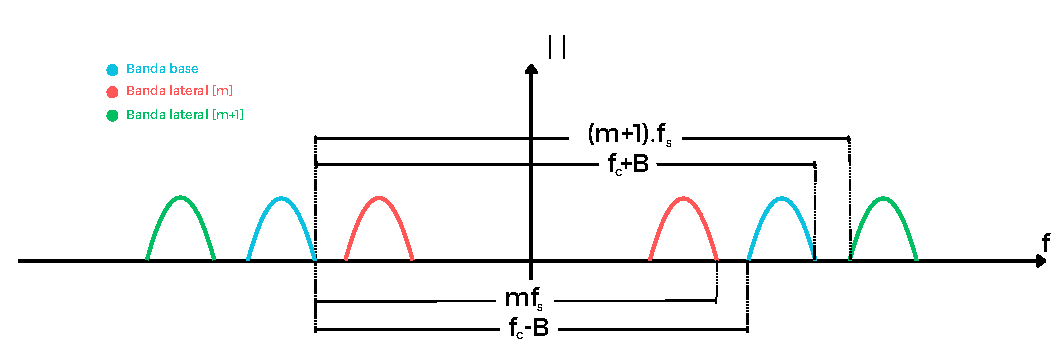
\includegraphics[width = \textwidth]{Imagenes/7_Sub_nyq/limites.pdf}
  \caption{Visualización de límites.}
  \label{fig: visualizacion de limites}
\end{figure}

\noindent de este modo:

\begin{equation}
    [{{f_s}^m}_{min};{{f_s}^m}_{max}] = \left[{{f_s}^m}_{min} = \frac{2\cdot f_c + B}{m+1};\frac{2 \cdot f_c - B}{m}\right]
\end{equation}

\newpage
\subsection{Intervalos}
A partir del análisis previo es posible determinar los diferentes intervalos donde no se produce aliasing para la señal solicitada. Considerar que los m válidos para el muestreo sub-Nyquist corresponde con $m\in \{ 1,2\}$ ($m_{val} = [35.28kHz/14kHz + 1/2] = 2$), por lo que los dos posible intervalos son:

\vspace{0.5cm}
\begin{table}[H]
\centering{
\begin{tabular}{c c c}
\toprule
$m$ & $f_{s,\min}^{(m)}$ [kHz] & $f_{s,\max}^{(m)}$ [kHz] \\
\midrule
1 & 42.28 & 56.56 \\
2 & 28.19 & 28.28 \\
\bottomrule
\end{tabular}
}
\caption{Intervalos de muestreo sin aliasing (muestreo sub-Nyquist)}
\label{tab: subnyquist}
\end{table}
\subsection{Verificación empírica}
Con tal de verificar el desarrollo teórico, se realizaron mediciones en las condiciones especificadas:
\begin{figure}[H]
    \centering
    \begin{subfigure}{0.48\textwidth}
        \centering
        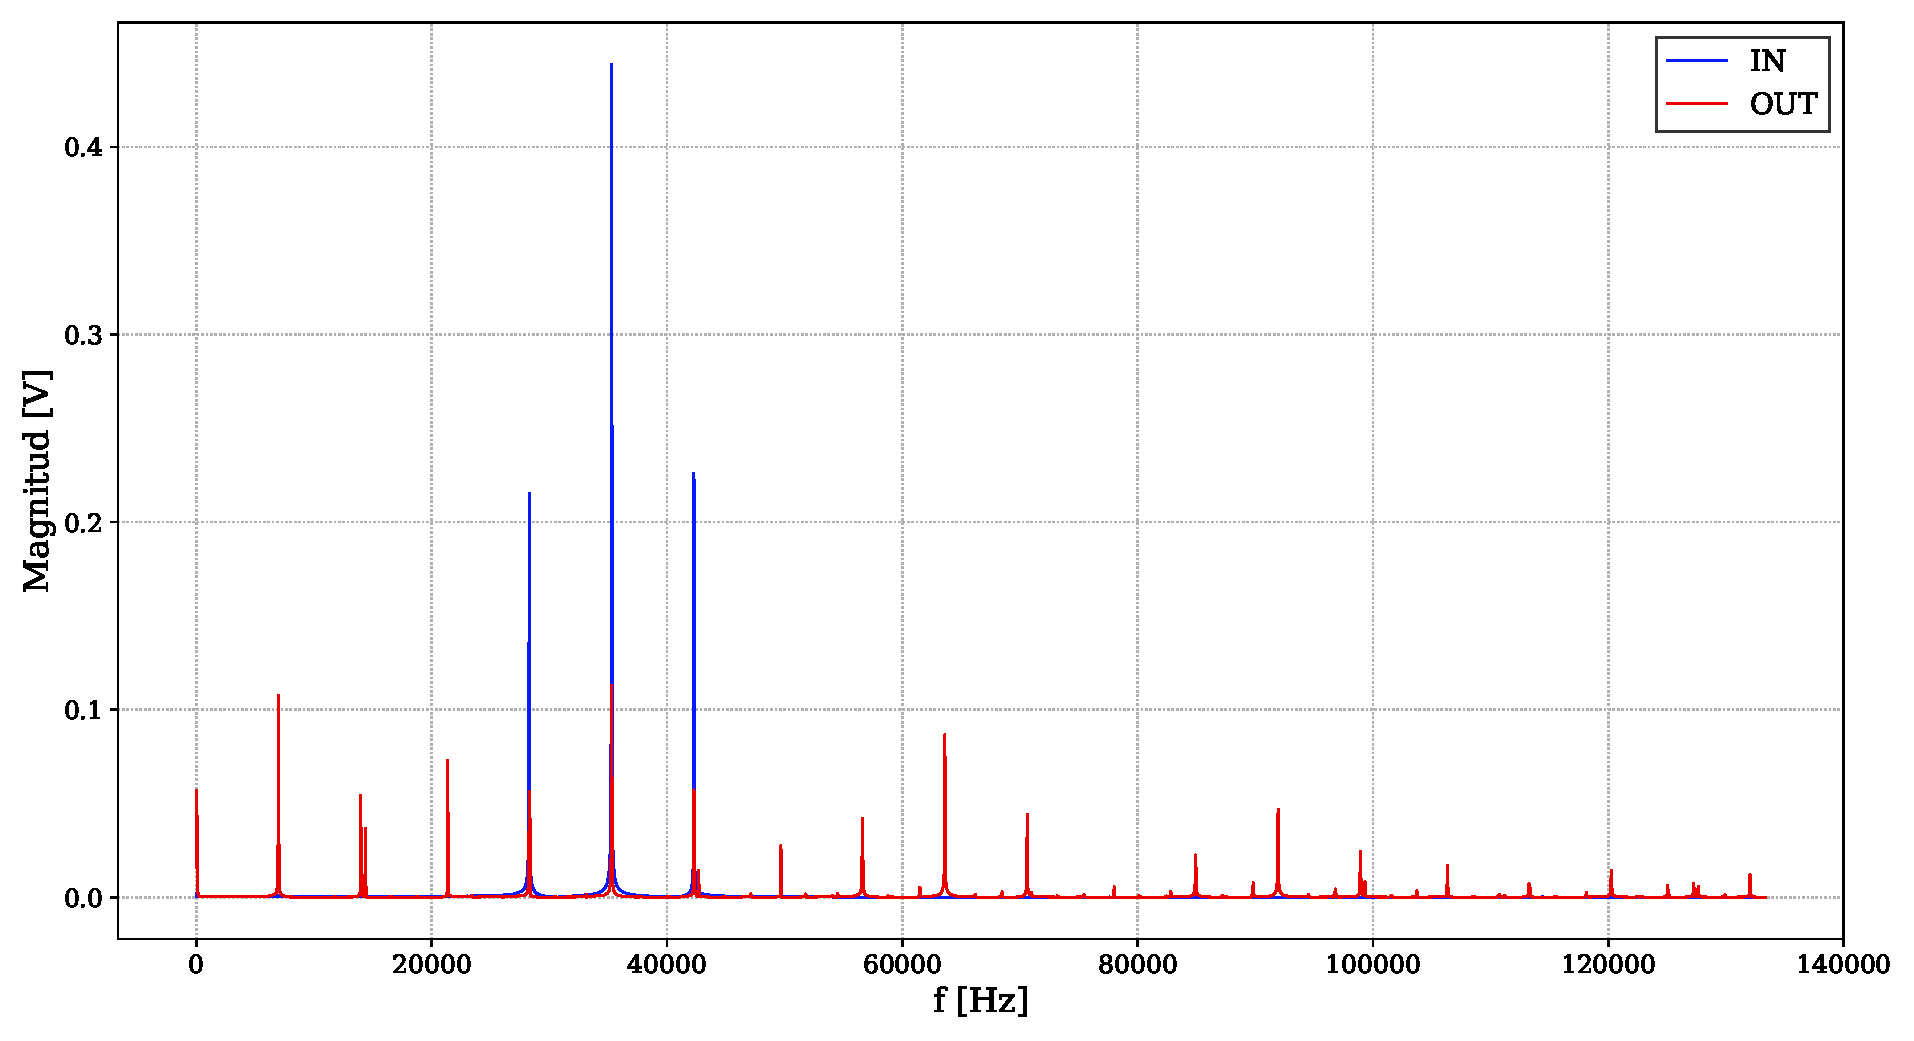
\includegraphics[width=\textwidth]{Imagenes/7_Sub_nyq/nat_fs_28k_D_25.pdf}
        \caption{Muestreo natural, $D=25\%$}
    \end{subfigure}
    \hfill
    \begin{subfigure}{0.48\textwidth}
        \centering
        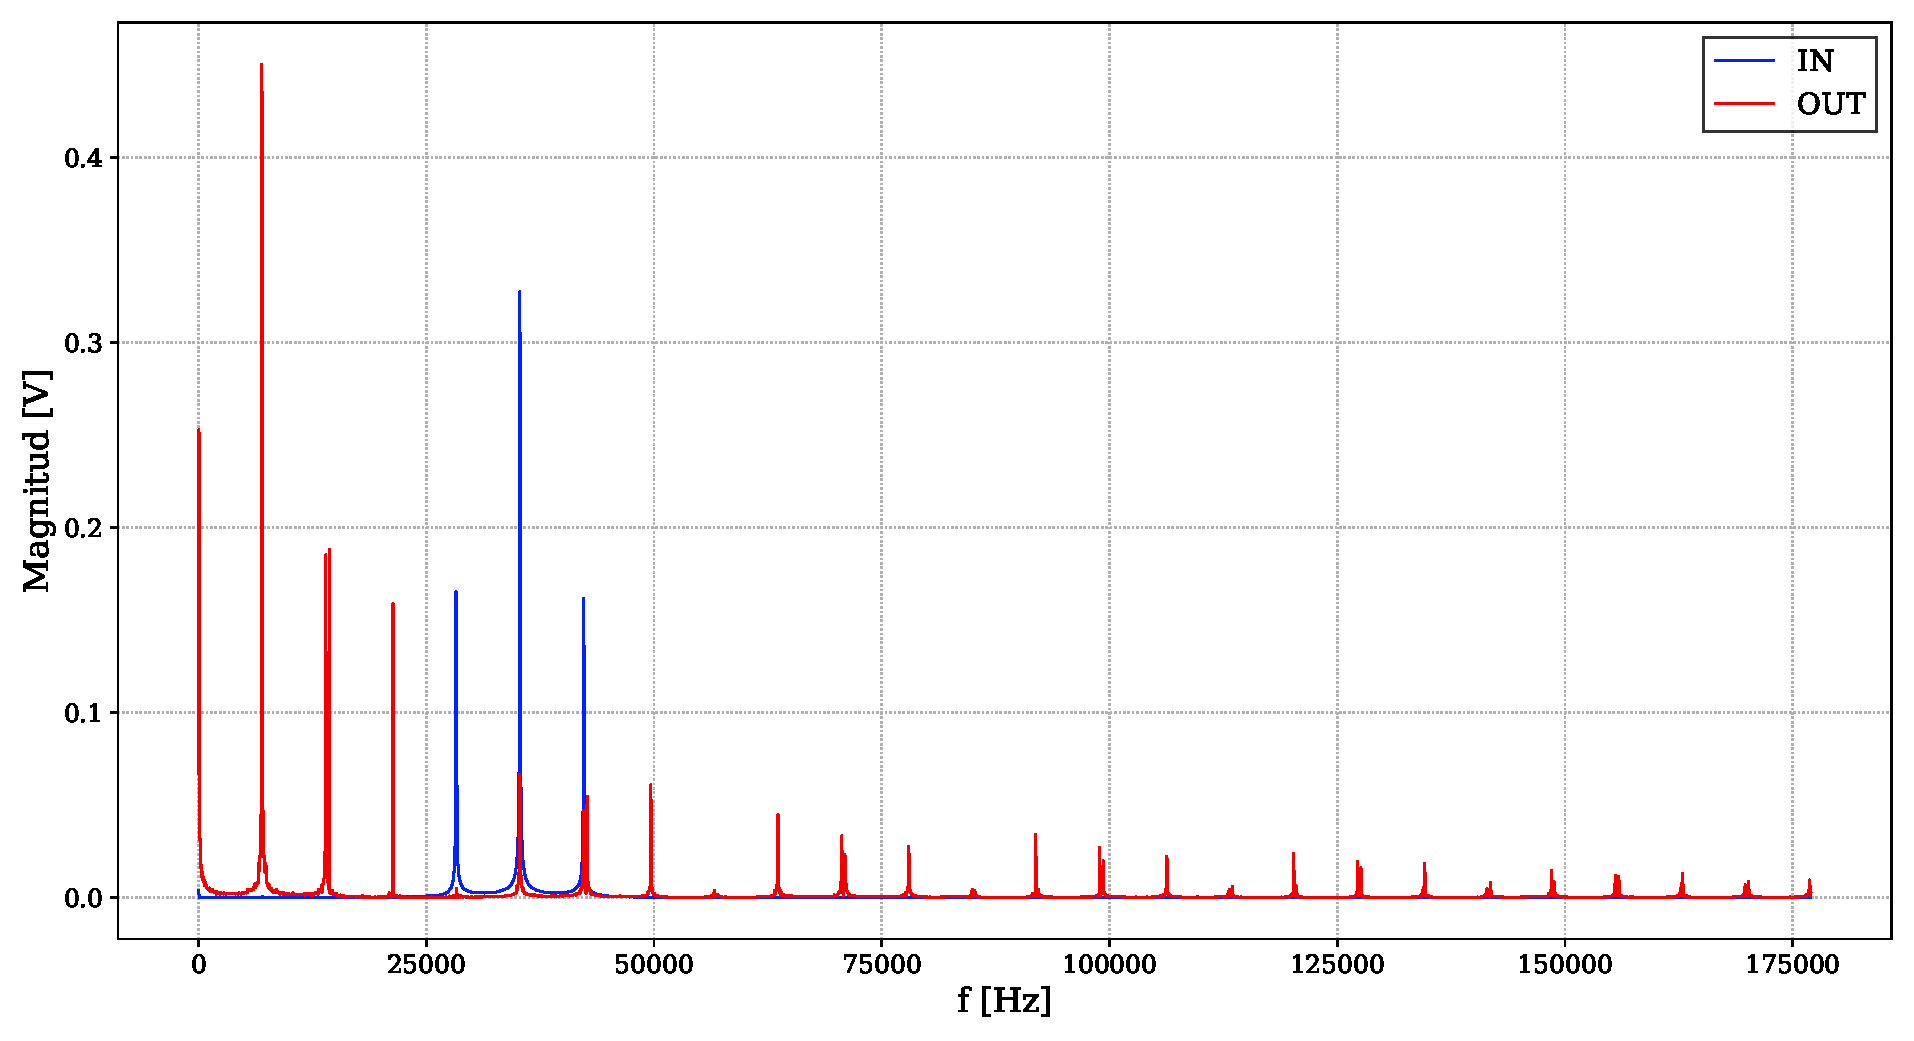
\includegraphics[width=\textwidth]{Imagenes/7_Sub_nyq/SH_fs_28k_D_5.pdf}
        \caption{Sample \& Hold, $D=5\%$}
        \label{fig: 7 28k SH}
    \end{subfigure}
    \caption{Mediciones para $f_s = 28\,\text{kHz}$.}
\end{figure}


\begin{figure}[H]
    \centering
    \begin{subfigure}{0.48\textwidth}
        \centering
        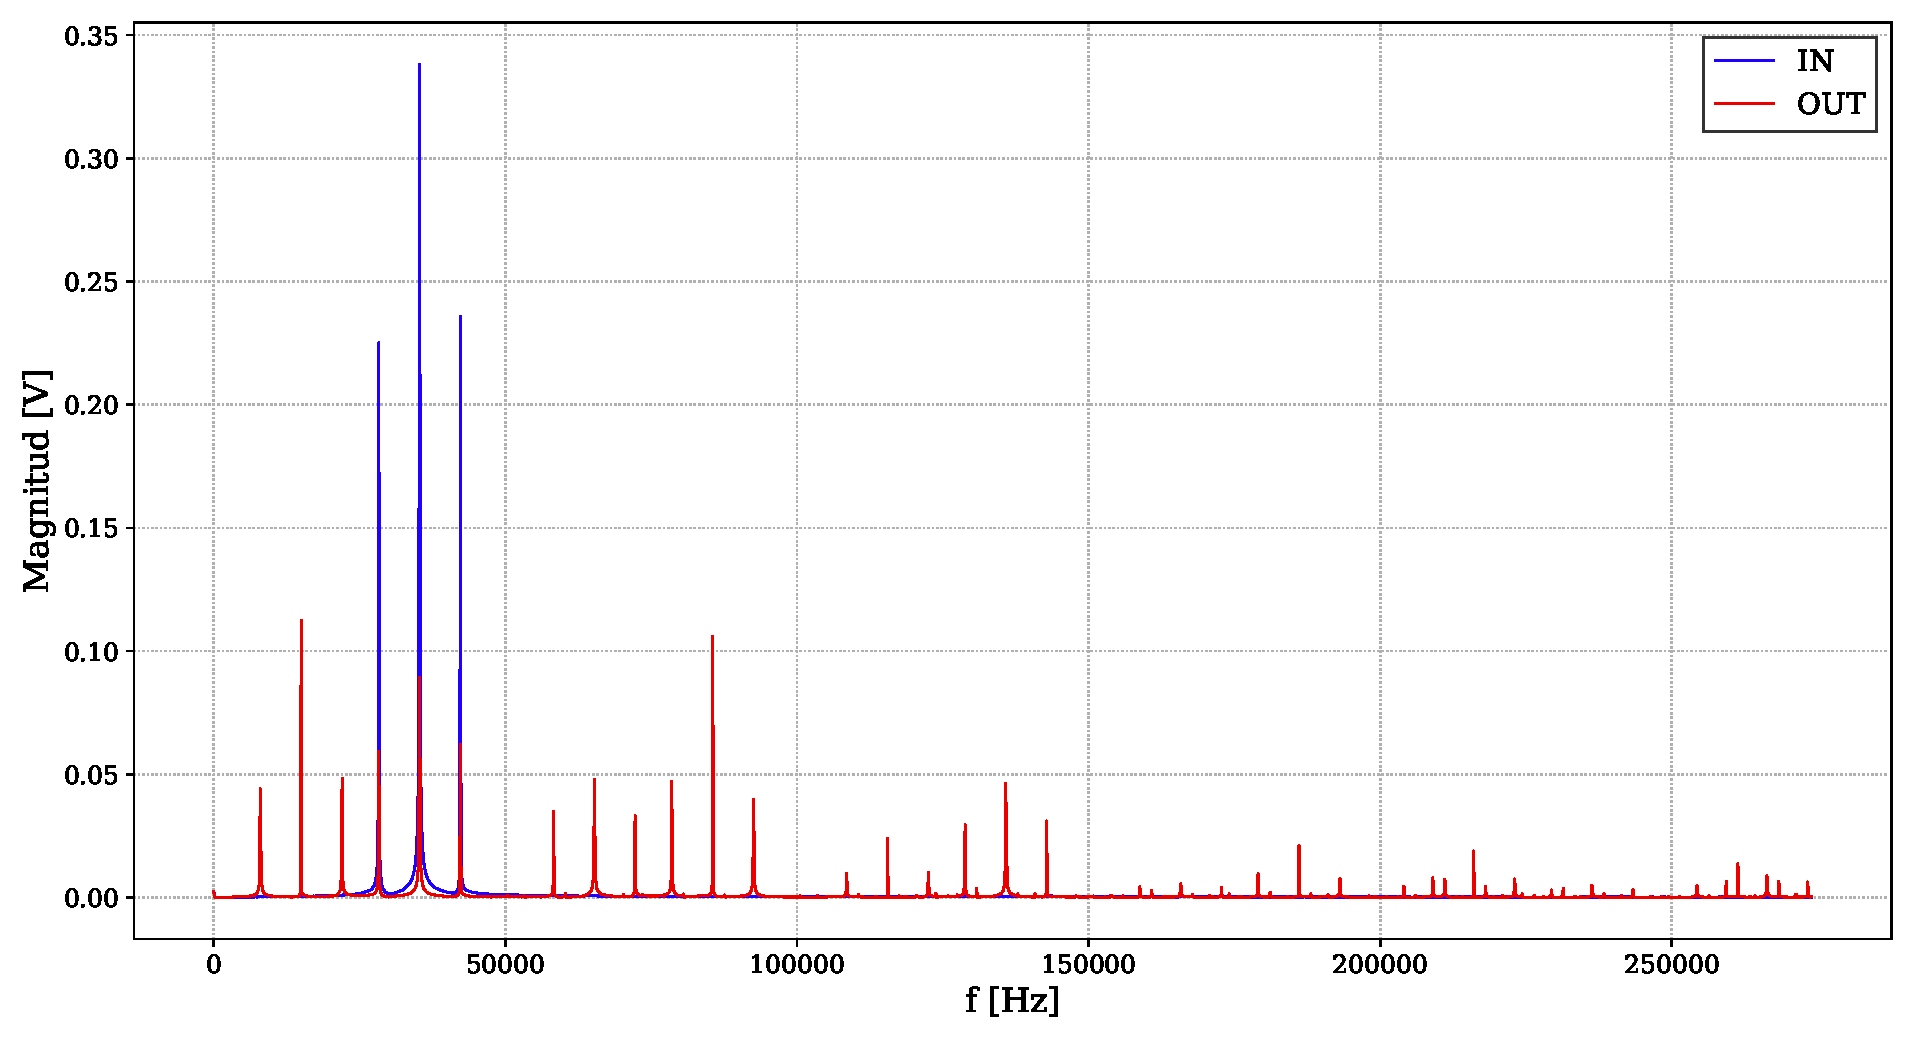
\includegraphics[width=\textwidth]{Imagenes/7_Sub_nyq/nat_fs_50k_D_25.pdf}
        \caption{Muestreo natural, $D=25\%$}
    \end{subfigure}
    \hfill
    \begin{subfigure}{0.48\textwidth}
        \centering
        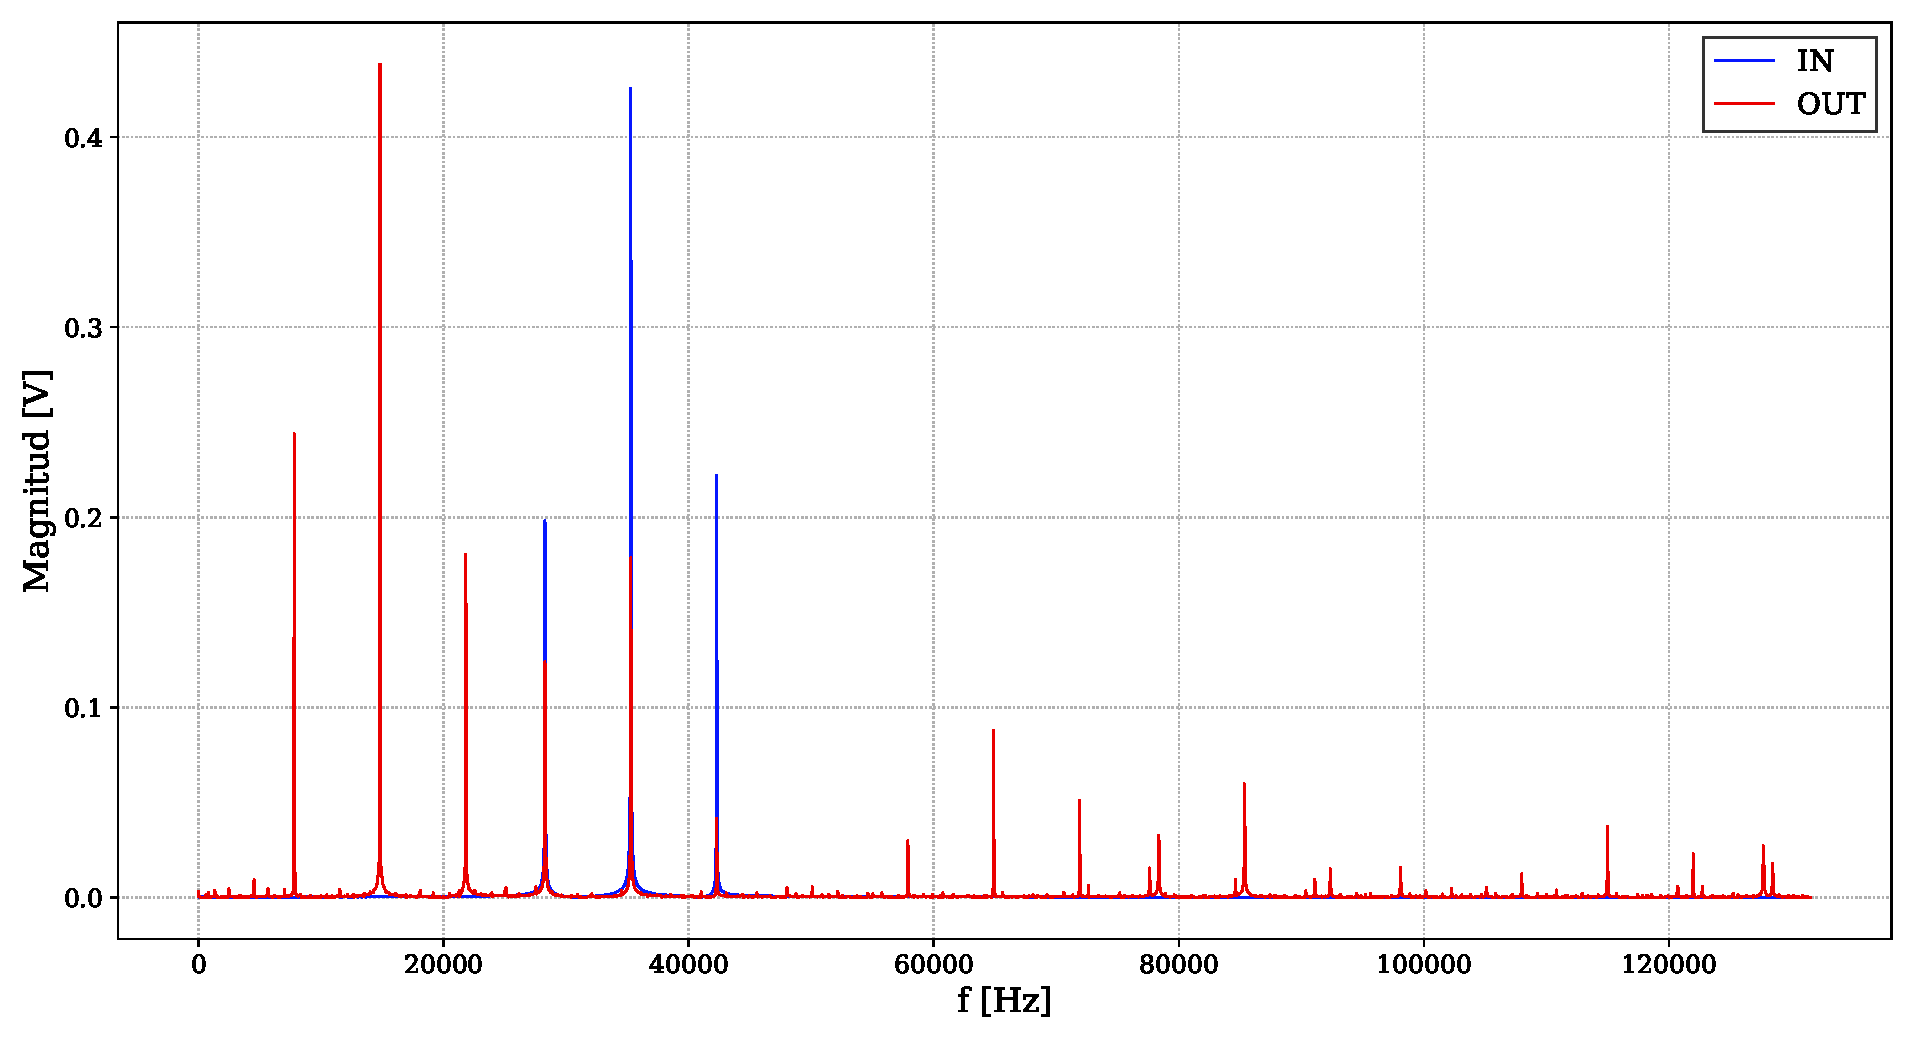
\includegraphics[width=\textwidth]{Imagenes/7_Sub_nyq/SH_fs_50k_D_5.pdf}
        \caption{Sample \& Hold, $D=5\%$}
    \end{subfigure}
    \caption{Mediciones para $f_s = 50\,\text{kHz}$.}
\end{figure}


\noindent donde se observa un comportamiento satisfactorio (se observan la cantidad de réplicas esperadas sin alias).

\subsection{Comportamiento en de la configuración de muestreo}
En las Figuras de la sección anterior se observaron diferencias, de acuerdo al tipo de muestreo. Esto resulta razonable en función de las relaciones encontradas en el ejercicio 5. Por un lado el muestreo natural sigue la relación:

\begin{align*}
    Y(f) =  X(f) * \sum_{n \in \mathbb{Z}} 
D \cdot sinc(nD) \cdot e^{-j2\pi nD/2} \cdot \delta(f-nf_s)
\end{align*}

\noindent mientras que el muestreo con S\&H dispone de la expresión:


\begin{align*}
Y(f) &= Y_{inst} - Y_{nat} =  \left[X(f) * \sum_{n \in \mathbb{Z}} \delta(f-nf_s)\right] 
\cdot D_{hold} \cdot sinc(D_{hold} f/f_s) \cdot e^{-j2\pi D_{hold} f/2f_s} \\
&- X(f) * \sum_{n \in \mathbb{Z}} 
D \cdot sinc(nD_{sample}) \cdot e^{-j2\pi nD_{sample}/2} \cdot \delta(f-nf_s)
\end{align*}

De este modo, el muestreo natural presenta una modulación dependiente de la base de origen de las réplicas, que a su vez varia como función del duty. En este caso particular la sinc decae lentamente debido al duty del 25\% (al igual que todo el espectro se ve escalado por este factor).

Por otro lado el muestreo con S\&H puede aproximarse al de un muestreo instantáneo, dado que el término asociado al muestreo natural dispone del factor $D_{sample}=0.05$, mientras que el asociado al muestreo instantáneo $D_{hold}=0.95$. De este modo se espera que la amplitud de los armónicos este dada en función de la modulación de la sinc, ahora dependiente de la frecuencia. Este hecho se ve particularmente en el hecho de que los armónicos más cercanos al origen tiene mayor amplitud. Por otro lado, en el caso de $f_s = 28kHz$, se dispone de un cero de la sinc en $f = 29.47kHz$, el cual se puede apreciar con claridad en la Figura \ref{fig: 7 28k SH}.

Si variamos el duty de ambas configuraciones a un $50\%$ se observa:


\begin{figure}[H]
    \centering
    \begin{subfigure}{0.48\textwidth}
        \centering
        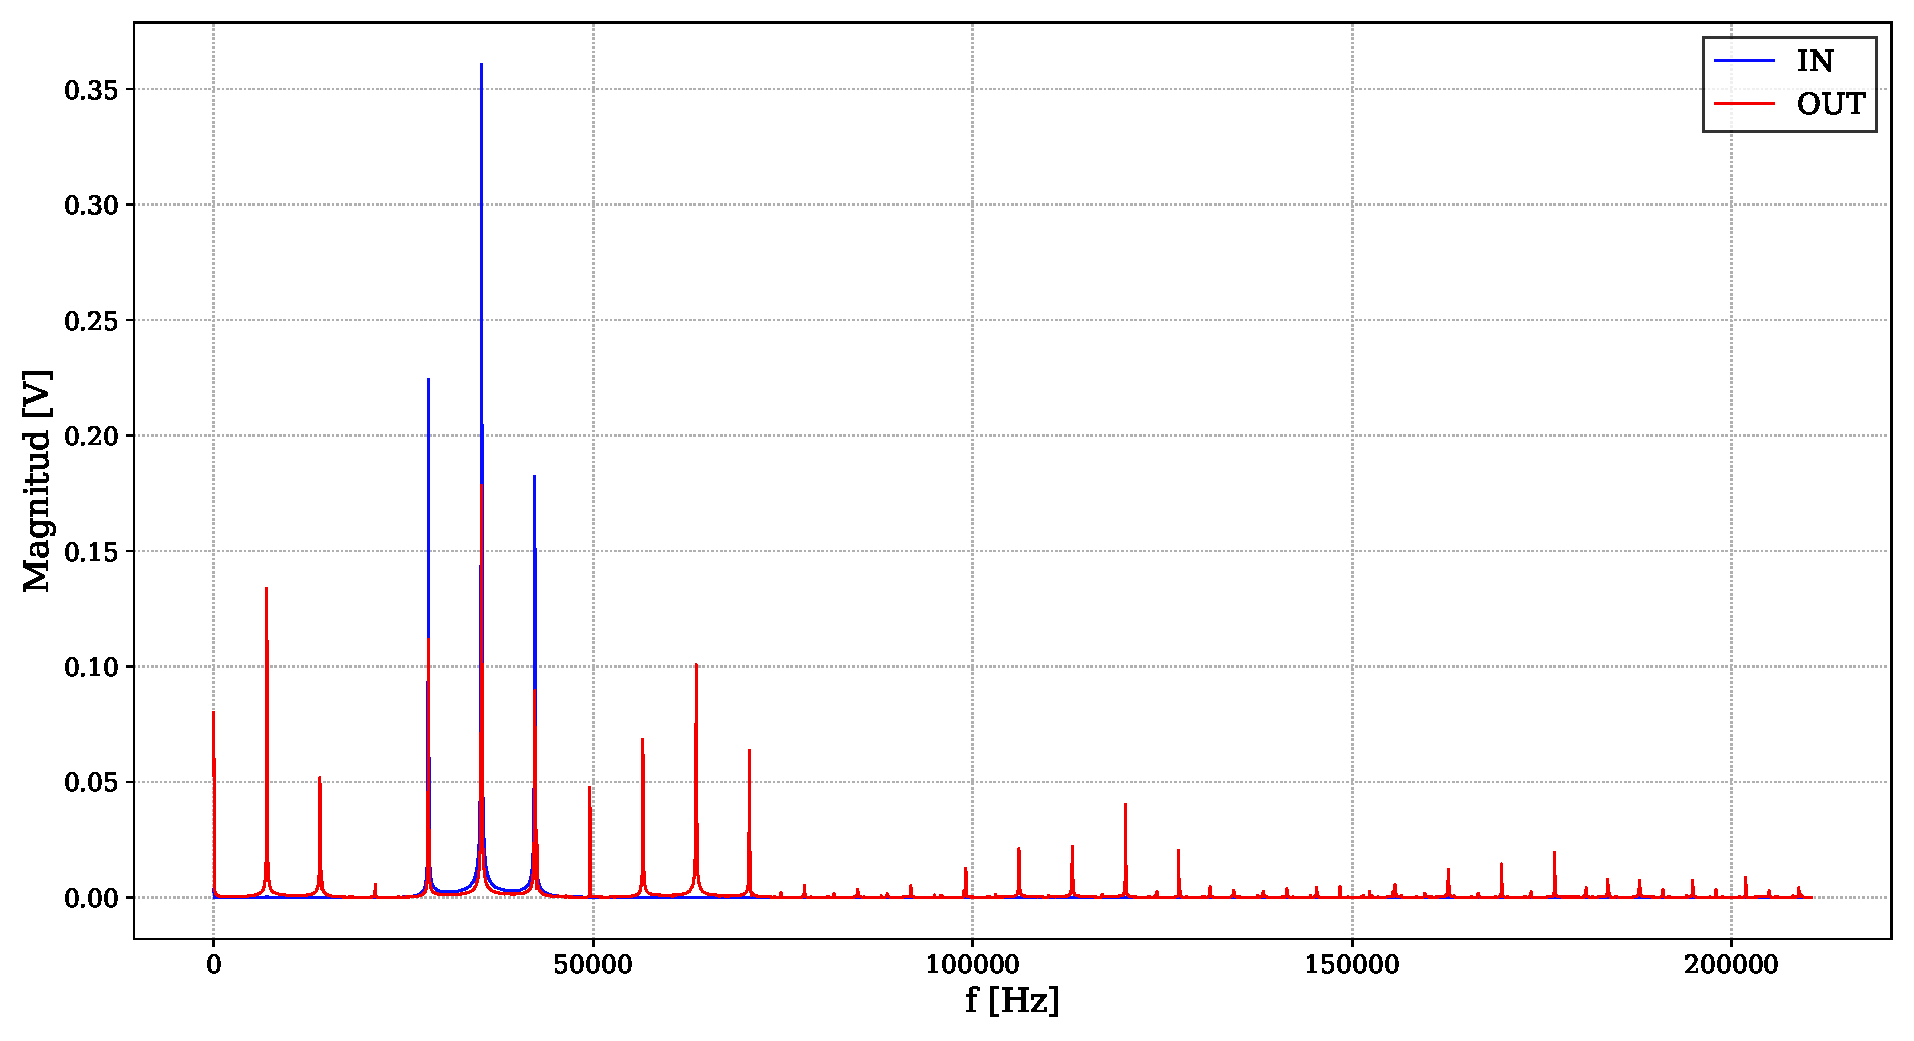
\includegraphics[width=\textwidth]{Imagenes/7_Sub_nyq/nat_fs_28k_D_50.pdf}
        \caption{Muestreo natural}
    \end{subfigure}
    \hfill
    \begin{subfigure}{0.48\textwidth}
        \centering
        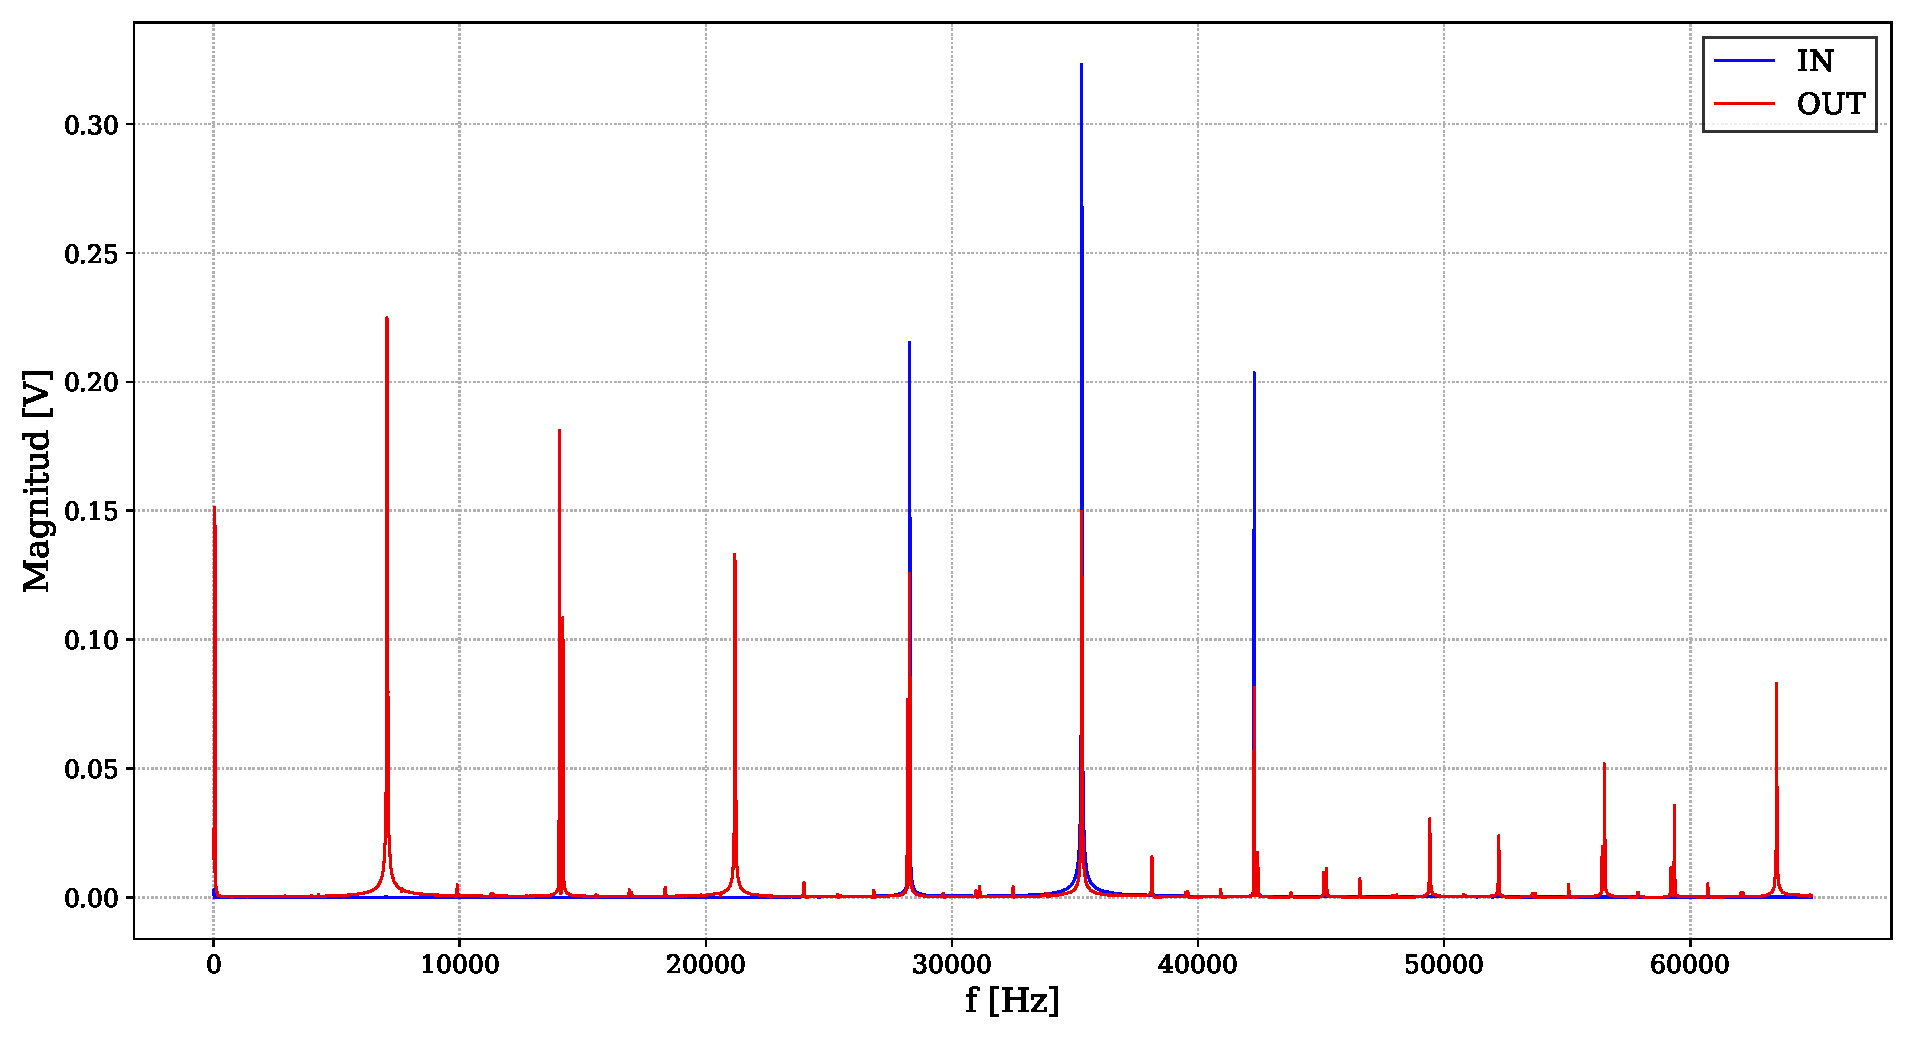
\includegraphics[width=\textwidth]{Imagenes/7_Sub_nyq/SH_fs_50k_D_50.pdf}
        \caption{Sample \& Hold}
    \end{subfigure}
    \caption{Mediciones para $f_s = 28\,\text{kHz}$ y $D = 50\%$.}
\end{figure}


\noindent lo cual confirma el comportamiento esperado. El caso del S\&H se complejiza dado que ambas componentes aportan significativamente; sin embargo, se puede destacar, por ejemplo, que el aumento de la amplitud de las componentes provenientes de la banda base como función del aumento de $D_{sample}$ resulta notorio.
